\usetikzlibrary{calc,positioning}
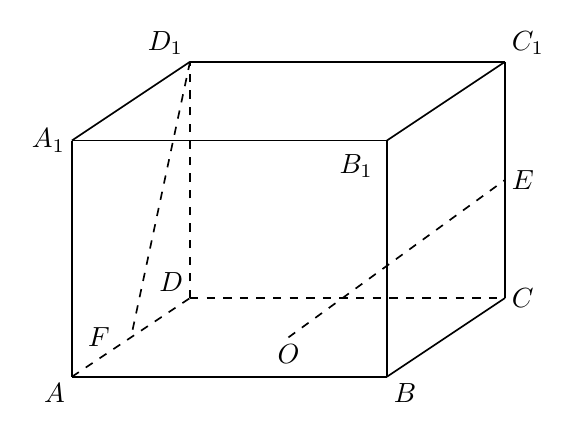
\begin{tikzpicture}[x=1cm,y=1cm,line width=.6pt,font=\normalsize,
 geometry edge/.style={solid,line width=.6pt,draw=black},
 geometry label/.style={font=\normalsize,inner sep=1.5pt,outer sep=1pt,draw=none}]

\coordinate (A) at (0,0);
\coordinate (B) at (4,0);
\coordinate (C) at (5.5,1);
\coordinate (D) at (1.5,1);
\coordinate (A1) at (0,3);
\coordinate (B1) at (4,3);
\coordinate (C1) at (5.5,4);
\coordinate (D1) at (1.5,4);
\coordinate (O) at (2.75,0.5);
\coordinate (E) at (5.5,2.5);
\coordinate (F) at (0.75,0.5);
\draw[geometry edge] (A)--(B);
\draw[geometry edge] (B)--(B1);
\draw[geometry edge] (B1)--(A1);
\draw[geometry edge] (A1)--(A);
\draw[geometry edge] (B1)--(C1);
\draw[geometry edge] (C1)--(D1);
\draw[geometry edge] (D1)--(A1);
\draw[geometry edge] (C1)--(C);
\draw[geometry edge] (B)--(C);
\draw[geometry edge,dashed] (A)--(D);
\draw[geometry edge,dashed] (D)--(C);
\draw[geometry edge,dashed] (D)--(D1);
\draw[geometry edge,dashed] (D1)--(F);
\draw[geometry edge,dashed] (O)--(E);
\node[geometry label,below left] at (A) {$A$};
\node[geometry label,below right] at (B) {$B$};
\node[geometry label,right] at (C) {$C$};
\node[geometry label,above left] at (D) {$D$};
\node[geometry label,left] at (A1) {$A_{1}$};
\node[below left=2pt] at (B1) {$B_{1}$};
\node[geometry label,above right] at (C1) {$C_{1}$};
\node[geometry label,above left] at (D1) {$D_{1}$};
\node[geometry label,below] at (O) {$O$};
\node[geometry label,right] at (E) {$E$};
\node[left=2pt,xshift=-2.00bp,yshift=0.00bp] at (F) {$F$};
\end{tikzpicture}
